\input{.template/template.tex}

\begin{document}

\makeheader{end of contest}

Floatworld is inhabited by protons and electrons.
 Although they have always lived in peace, they live strictly separated because of the life threatening conditions on floatworld. 
 The surface is mostly covered by positive (+) and negative (-) loaded tiles.
 Electrons float above negative and protons float above positive loaded surface. 
 For unknown reasons there are patches (0) that are neither positive nor negative where none can float. 
 When the protons and electrons stop floating, they hit the ground and die horribly!  
 When protons and electrons get to close to one another they will be pulled together, stop floating and die horribly as well! (at least not alone). 
 The surface looks like a grid and the protons and electrons can float to adjacent tiles that are properly loaded. 
 They can move vertical, horizontal, and diagonal. 
 Diagonal crossings, where positive and negative loaded tiles are next to each other, are very dangerous. 
 Only the biggest and strongest protons or electrons should cross them, but it is still possible and they count as adjacent! 
 It is possible that not all the properly loaded tiles on floatworld are reachable for all electrons and protons. 
 Because of some weird circumstances it is possible that floatworld is uninhabitable by protons and/or electrons! 
 What is the largest area (number of tiles) that a proton or electron can float if it was born in the right area in floatworld?

\paragraph*{Input}

The inputs first line contains $w$ and $h$ $(1 \leq w, h \leq 1000)$, the width and height of floatworld. The next $h$ lines contain $w$ characters (+, -, 0) which represent the surface of floatworld.

\paragraph*{Output}

Print one line containing $p$ and $e$ $(p,e \leq 10^6)$ representing the largest area of the protons ($p$) and electrons ($e$).


\begin{samples}
  \sample{sample1}
  \sample{sample2}
  \sample{sample3}
\end{samples}

\begin{tabular}{cc}
  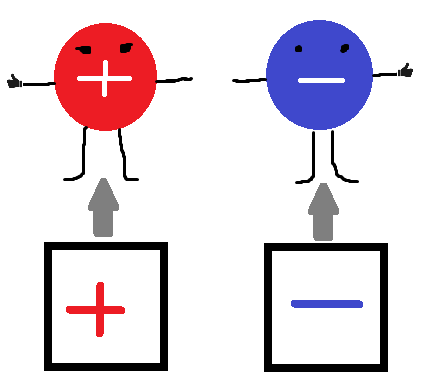
\includegraphics[width=0.5\textwidth]{../../floating.png}
    & 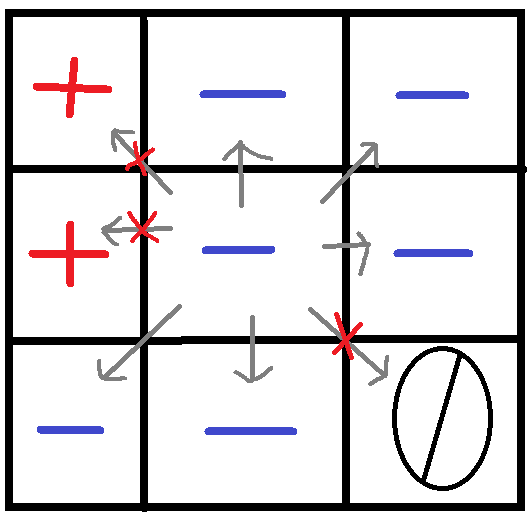
\includegraphics[width=0.5\textwidth]{../../grid.png} \\
  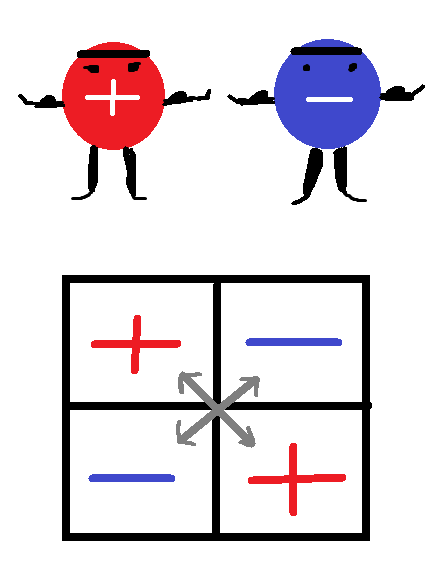
\includegraphics[width=0.5\textwidth]{../../crossing.png}
    & 
\includegraphics[width=0.35\textwidth]{../../rip.png} \\
\end{tabular}


\end{document}
